\documentclass{article}
\usepackage{graphicx} % Required for inserting images
\usepackage[margin=1in]{geometry}
\usepackage{amsmath}
\usepackage{amsthm}
\usepackage{amssymb}
\usepackage{amsfonts}
\usepackage{verbatim}
\usepackage{tikz}
\usepackage{xcolor}

\title{Final Project: Report}
\author{Dante Buhl}


\DeclareMathOperator{\cond}{cond}
\DeclareMathOperator{\vecspan}{span}
\DeclareMathOperator{\sign}{sign}
\DeclareMathOperator{\diag}{diag}
\DeclareMathOperator{\upper}{upper}
\DeclareMathOperator{\lowtri}{lower}

\begin{document}

\newcommand{\bs}[1]{\boldsymbol{#1}}
\newcommand{\bmp}[1]{\begin{minipage}{#1\textwidth}}
\newcommand{\emp}{\end{minipage}}
\newcommand{\R}{\mathbb{R}}
\newcommand{\C}{\mathbb{C}}
\newcommand{\N}{\mathcal{N}}
\newcommand{\I}{\mathrm{I}}
\newcommand{\K}{\bs{\mathrm{K}}}
\newcommand{\m}{\bs{\mu}_*}
\newcommand{\s}{\bs{\Sigma}_*}
\newcommand{\dt}{\Delta t}
\newcommand{\tr}[1]{\text{Tr}(#1)}
\newcommand{\Tr}[1]{\text{Tr}(#1)}

\maketitle



\section{Part A: Reduced Rank Image Reconstruction}
\begin{enumerate}
    
    \item

    The first ten largest singular values are $\{ ... \}$. Furthermore the ``rest singular values'' are as follows $\{ \sigma_{10} = , \sigma_{20} = , \sigma_{40} = , \sigma_{80} = , \sigma_{160} = , \sigma_{320} = , \sigma_{640} = , \sigma_{1279} = \}$. 

    \item Here are the following eight images generated by the reduced rank approximation for the image. 

\begin{center}
    
    \begin{tabular}{| c | c |}
    \hline \\
    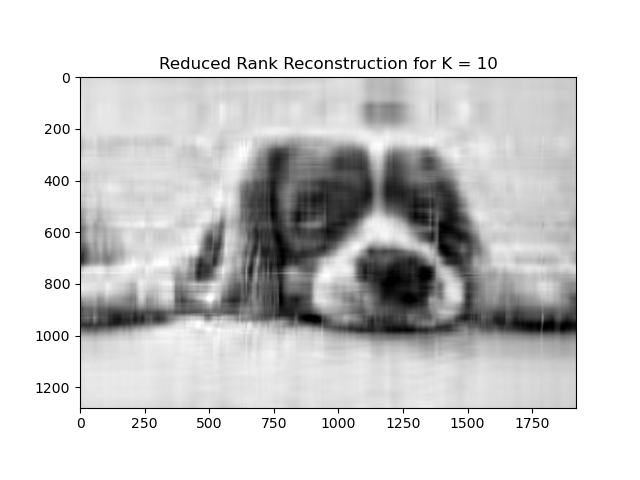
\includegraphics[width=.40\textwidth]{Image_appn_100010.png} & 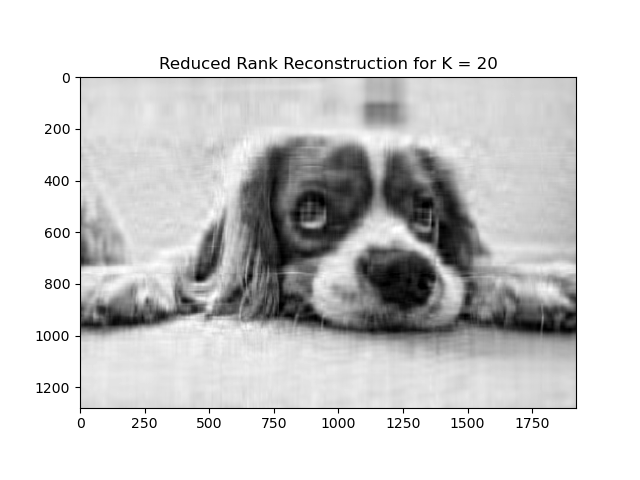
\includegraphics[width=.40\textwidth]{Image_appn_100020.png} \\
    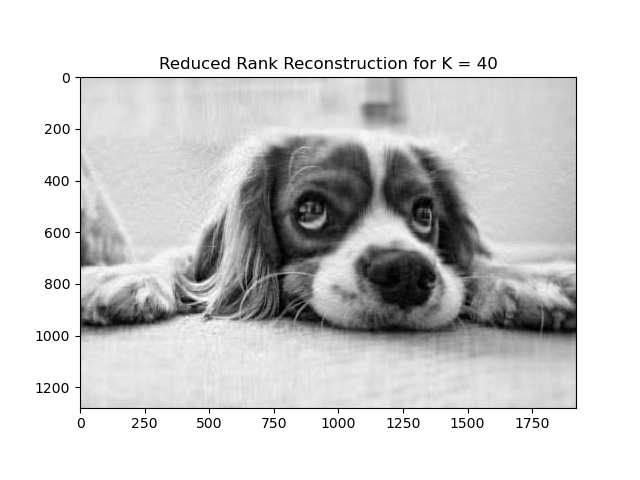
\includegraphics[width=.40\textwidth]{Image_appn_100040.png} & 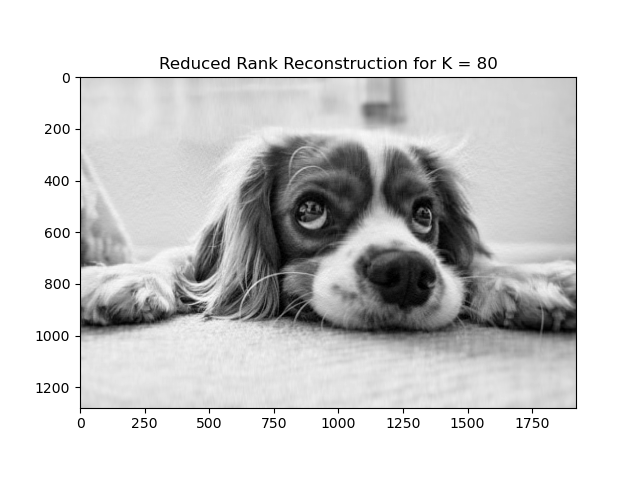
\includegraphics[width=.40\textwidth]{Image_appn_100080.png} \\
    \hline
    \end{tabular}

    \begin{tabular}{| c | c |}
    \hline \\
    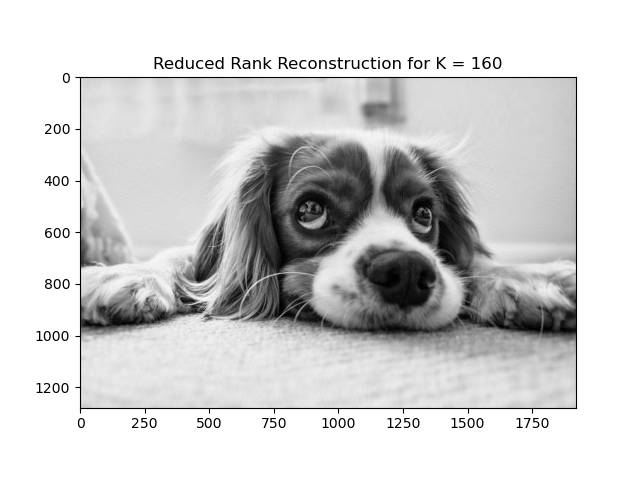
\includegraphics[width=.40\textwidth]{Image_appn_100160.png} & 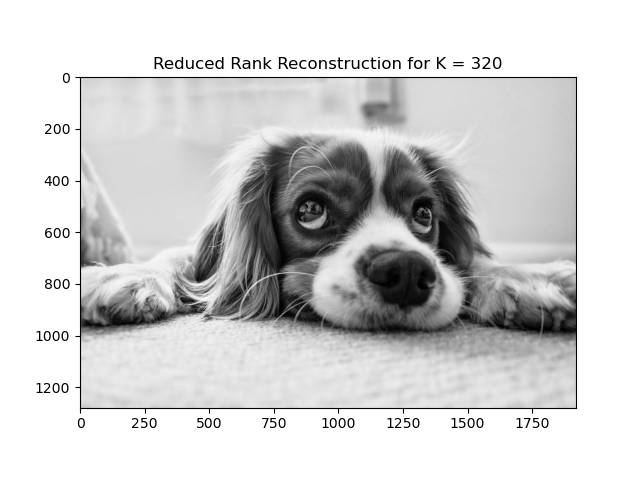
\includegraphics[width=.40\textwidth]{Image_appn_100320.png} \\
    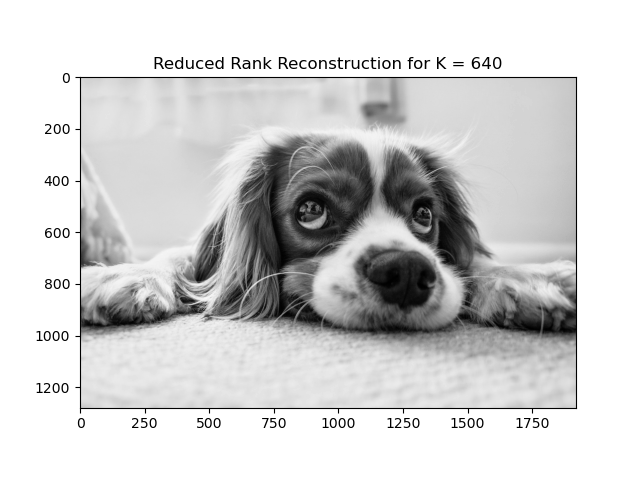
\includegraphics[width=.40\textwidth]{Image_appn_100640.png} & 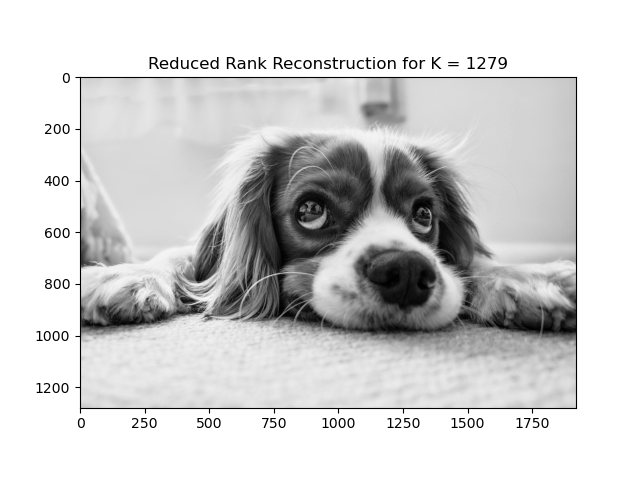
\includegraphics[width=.40\textwidth]{Image_appn_101279.png} \\
    \hline
    \end{tabular}

    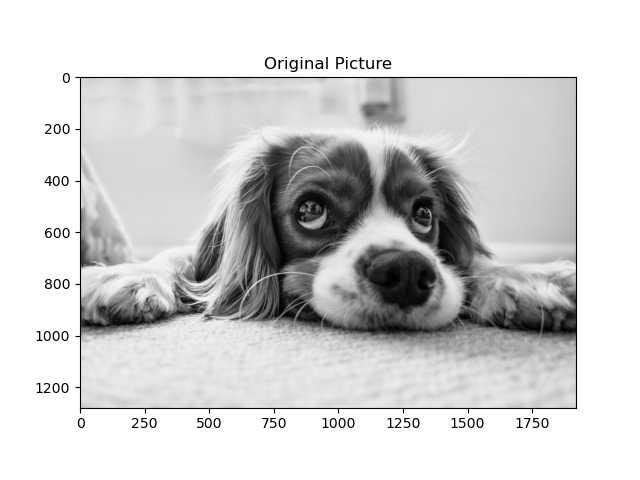
\includegraphics[width=.60\textwidth]{original.png}
\end{center}

    \item 

    It is easily noticable that as we reduce the rank of our appoximations more and more, that the quality of the image decreases. Some of the differences between rank approximations aren't as noticable as others. Between ranks of the reconstruction 40 and 80 there is a very noticable sacrifice in image quality. There seem to be smudges in the picture and a sort of typical graininess which is present in low resolution images. This is what is noticable here. Looking at the error reports of these approximations we find that we only find a normalized error below $10^{-3}$ for our rank 10 approximation. All other normalized errors are of order $10^{-3}$ or lower. The lowest being the rank 1279 error at $10^{-16}$ exactly the order of machine double precision. 

\end{enumerate}

\section{Iterative Methods}
\subsection{Gauss-Jacobi/Gauss-Seidel}

    \begin{enumerate}

        \item Both the Gauss-Jacobi and Gauss-Seidel methods involve an iterative method in which we recompute a vector x and after (hopefully) a finite number of iterations we will reach the desired level of error. They differ in the compution of the next x vector from the proceeding one. In Gauss-Jacobi, it is simply one line of matrix multiplcation and subtraction, i.e.
    \[
        x^{(n)} = D^{-1}(b - Rx^{(n-1)}), \quad D = \diag(A), \quad R = A - D
    \]
    This is much easier to compute since $x^{(n)}$ only depends on the givens $A, D, R, b$ and the previous iteration. A slightly more complex algorithm, Gauss-Seidel, is derived from this where we break $R$ into an upper and lower matrix, i.e.
    \[
        A = D + R + L, \quad D = \diag(A), \quad R = \upper\Delta(A - D), \quad L = \lowtri\Delta(A - D)    
    \]
    Here the iterative method is 
    \[
        x^{(n)} = 0 \to x_i^{(n)} = \frac{1}{a_{ii}}(b_i - L_{i, 1:i-1}x_{1:i-1}^{(n)} - R_{i, i+1:m}x_{i+1:m}^{(n-1)})
    \]
    Here we have that going down the elements of $x^{(n)}$ each element depends on the term before it. This means that rather than one line of matrix opertions, we have to express the iterative process for $x^{(n)}$ as a loop over the $m$ elements of the vector. 

    \item

    Here are the plots obtained for all values of D. 

    \item 
        
    Some of the cases didn't converge, specifically $D = 2$ and $D = 5$ for the Gauss-Jacobi method. For both of these cases the number of iterations reached into the order of $10^2$ and the final result is NaN, usually indicating an underflow. For the cases where both methods converge, we see that Gauss-Seidel converges more quickly. This matches the theoretical predictions that we went over in lecture yielding better convergence and stability for Gauss-Seidel with the trade off of not being able to parallelize. 

    \item 
    For the case of $A_{ii} = i$ we have that the Gauss-Jacobi method does not converge, but Gauss-Seidel does. 

    \end{enumerate}

\subsection{Conjugate Gradient}

    \begin{enumerate}

        \item The Conjugate Gradient Method is a method which 
    
        \item \colorbox{yellow}{DON'T FORGET TO WRITE THE DAMN PROOF}

        \item This method converges very quickly and with high accuracy for each value of D! In the table below we have the number of iterations needed to converge to order $10^{-5}$ accuracy (note that though the tolerance parameter is given as $10^{-5}$ we have that the actual value of the resultant error is below $10^{-14}$ in only 2 iterations). 

            \begin{center}

                \begin{tabular}{|c|c|c|c|c|c|}
                \hline
                $D = $ & 2 & 5 & 10 & 100 & 1000 \\
                \hline
                $N = $ & 2 & 2 & 2 & 2 & 2 \\
                \hline
                \end{tabular}

            \end{center}

        \item Specifically the Diagonal preconditioner is not strong for these matrices. The reason is that since each diagonal element is the same we are effectively dividing the whole matric by the same value, thereby not scaling the eigenvalues of $M^{-1}A$ in any significant manner whatsoever. 

        \item

        \item

    \end{enumerate}


\end{document}
